\documentclass[twoside]{book}

% Packages required by doxygen
\usepackage{fixltx2e}
\usepackage{calc}
\usepackage{doxygen}
\usepackage[export]{adjustbox} % also loads graphicx
\usepackage{graphicx}
\usepackage[utf8]{inputenc}
\usepackage{makeidx}
\usepackage{multicol}
\usepackage{multirow}
\PassOptionsToPackage{warn}{textcomp}
\usepackage{textcomp}
\usepackage[nointegrals]{wasysym}
\usepackage[table]{xcolor}

% Font selection
\usepackage[T1]{fontenc}
\usepackage[scaled=.90]{helvet}
\usepackage{courier}
\usepackage{amssymb}
\usepackage{sectsty}
\renewcommand{\familydefault}{\sfdefault}
\allsectionsfont{%
  \fontseries{bc}\selectfont%
  \color{darkgray}%
}
\renewcommand{\DoxyLabelFont}{%
  \fontseries{bc}\selectfont%
  \color{darkgray}%
}
\newcommand{\+}{\discretionary{\mbox{\scriptsize$\hookleftarrow$}}{}{}}

% Page & text layout
\usepackage{geometry}
\geometry{%
  a4paper,%
  top=2.5cm,%
  bottom=2.5cm,%
  left=2.5cm,%
  right=2.5cm%
}
\tolerance=750
\hfuzz=15pt
\hbadness=750
\setlength{\emergencystretch}{15pt}
\setlength{\parindent}{0cm}
\setlength{\parskip}{3ex plus 2ex minus 2ex}
\makeatletter
\renewcommand{\paragraph}{%
  \@startsection{paragraph}{4}{0ex}{-1.0ex}{1.0ex}{%
    \normalfont\normalsize\bfseries\SS@parafont%
  }%
}
\renewcommand{\subparagraph}{%
  \@startsection{subparagraph}{5}{0ex}{-1.0ex}{1.0ex}{%
    \normalfont\normalsize\bfseries\SS@subparafont%
  }%
}
\makeatother

% Headers & footers
\usepackage{fancyhdr}
\pagestyle{fancyplain}
\fancyhead[LE]{\fancyplain{}{\bfseries\thepage}}
\fancyhead[CE]{\fancyplain{}{}}
\fancyhead[RE]{\fancyplain{}{\bfseries\leftmark}}
\fancyhead[LO]{\fancyplain{}{\bfseries\rightmark}}
\fancyhead[CO]{\fancyplain{}{}}
\fancyhead[RO]{\fancyplain{}{\bfseries\thepage}}
\fancyfoot[LE]{\fancyplain{}{}}
\fancyfoot[CE]{\fancyplain{}{}}
\fancyfoot[RE]{\fancyplain{}{\bfseries\scriptsize Generated by Doxygen }}
\fancyfoot[LO]{\fancyplain{}{\bfseries\scriptsize Generated by Doxygen }}
\fancyfoot[CO]{\fancyplain{}{}}
\fancyfoot[RO]{\fancyplain{}{}}
\renewcommand{\footrulewidth}{0.4pt}
\renewcommand{\chaptermark}[1]{%
  \markboth{#1}{}%
}
\renewcommand{\sectionmark}[1]{%
  \markright{\thesection\ #1}%
}

% Indices & bibliography
\usepackage{natbib}
\usepackage[titles]{tocloft}
\setcounter{tocdepth}{3}
\setcounter{secnumdepth}{5}
\makeindex

% Hyperlinks (required, but should be loaded last)
\usepackage{ifpdf}
\ifpdf
  \usepackage[pdftex,pagebackref=true]{hyperref}
\else
  \usepackage[ps2pdf,pagebackref=true]{hyperref}
\fi
\hypersetup{%
  colorlinks=true,%
  linkcolor=blue,%
  citecolor=blue,%
  unicode%
}

% Custom commands
\newcommand{\clearemptydoublepage}{%
  \newpage{\pagestyle{empty}\cleardoublepage}%
}

\usepackage{caption}
\captionsetup{labelsep=space,justification=centering,font={bf},singlelinecheck=off,skip=4pt,position=top}

%===== C O N T E N T S =====

\begin{document}

% Titlepage & ToC
\hypersetup{pageanchor=false,
             bookmarksnumbered=true,
             pdfencoding=unicode
            }
\pagenumbering{roman}
\begin{titlepage}
\vspace*{7cm}
\begin{center}%
{\Large Shape Demo }\\
\vspace*{1cm}
{\large Generated by Doxygen 1.8.11}\\
\end{center}
\end{titlepage}
\clearemptydoublepage
\tableofcontents
\clearemptydoublepage
\pagenumbering{arabic}
\hypersetup{pageanchor=true}

%--- Begin generated contents ---
\chapter{File Index}
\section{File List}
Here is a list of all files with brief descriptions\+:\begin{DoxyCompactList}
\item\contentsline{section}{srcs/\hyperlink{multiloc_8h}{multiloc.\+h} }{\pageref{multiloc_8h}}{}
\item\contentsline{section}{srcs/\hyperlink{utils_8h}{utils.\+h} }{\pageref{utils_8h}}{}
\end{DoxyCompactList}

\chapter{File Documentation}
\hypertarget{multiloc_8h}{}\section{multiloc.\+h File Reference}
\label{multiloc_8h}\index{multiloc.\+h@{multiloc.\+h}}
{\ttfamily \#include \char`\"{}Eigen/\+Dense\char`\"{}}\\*
{\ttfamily \#include $<$vector$>$}\\*
{\ttfamily \#include $<$iostream$>$}\\*
{\ttfamily \#include $<$fstream$>$}\\*
{\ttfamily \#include $<$iomanip$>$}\\*
{\ttfamily \#include $<$ctime$>$}\\*
{\ttfamily \#include $<$cmath$>$}\\*
{\ttfamily \#include $<$algorithm$>$}\\*
{\ttfamily \#include $<$sys/time.\+h$>$}\\*
Include dependency graph for multiloc.\+h\+:
\nopagebreak
\begin{figure}[H]
\begin{center}
\leavevmode
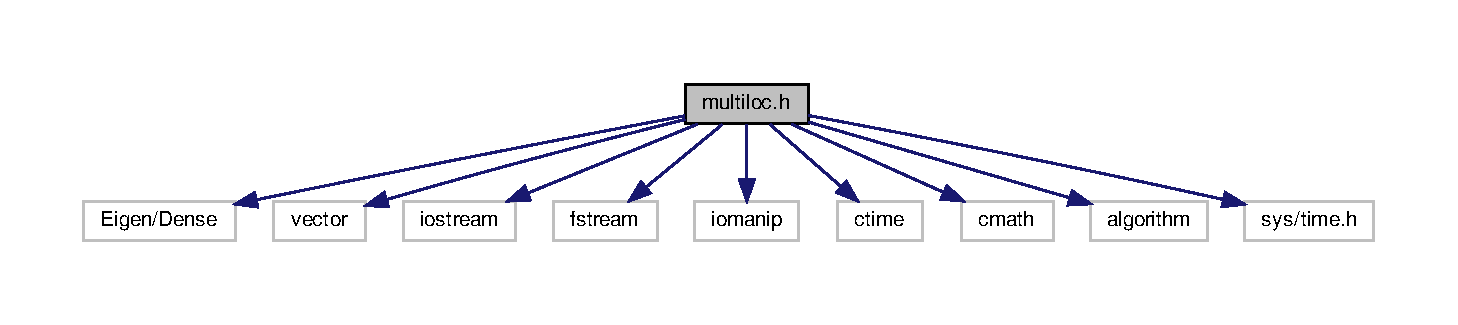
\includegraphics[width=350pt]{multiloc_8h__incl}
\end{center}
\end{figure}
This graph shows which files directly or indirectly include this file\+:
\nopagebreak
\begin{figure}[H]
\begin{center}
\leavevmode
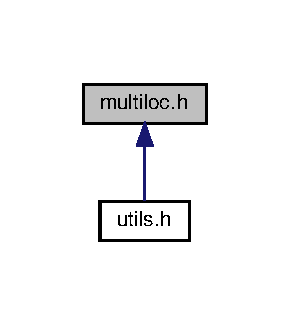
\includegraphics[width=139pt]{multiloc_8h__dep__incl}
\end{center}
\end{figure}
\subsection*{Typedefs}
\begin{DoxyCompactItemize}
\item 
typedef vector$<$ double $>$ \hyperlink{multiloc_8h_a490e31016ad1c0d99b23e323d64e3aac}{one\+\_\+\+Tuple}
\item 
typedef vector$<$ \hyperlink{multiloc_8h_a490e31016ad1c0d99b23e323d64e3aac}{one\+\_\+\+Tuple} $>$ \hyperlink{multiloc_8h_a2e41d128befae015727cbf20484696a9}{two\+\_\+\+Tuple}
\item 
typedef vector$<$ \hyperlink{multiloc_8h_a2e41d128befae015727cbf20484696a9}{two\+\_\+\+Tuple} $>$ \hyperlink{multiloc_8h_aa614d5a3aa93583e717bf9a9c9b6627b}{three\+\_\+\+Tuple}
\end{DoxyCompactItemize}
\subsection*{Functions}
\begin{DoxyCompactItemize}
\item 
void \hyperlink{multiloc_8h_ae92e2bd9031ed9ed66c58dfffcf01c94}{sortarry} (\hyperlink{multiloc_8h_a2e41d128befae015727cbf20484696a9}{two\+\_\+\+Tuple} \&list, int temp)
\begin{DoxyCompactList}\small\item\em 对一个二维的vector$<$vector$<$double$>$$>$的list进行按照每一个vector$<$double$>$的第2个元素进行升序 \end{DoxyCompactList}\item 
bool \hyperlink{multiloc_8h_ac6173a0dbaef919c983aba0501486521}{finditems} (double value, \hyperlink{multiloc_8h_a2e41d128befae015727cbf20484696a9}{two\+\_\+\+Tuple} \&list)
\begin{DoxyCompactList}\small\item\em 判断value元素是否属于2维vector中的第一个元素,如果value属于list中返回true,否则返回false. \end{DoxyCompactList}\item 
bool \hyperlink{multiloc_8h_ace45908ac4ee480fb56d3c9c75307948}{finditems} (double value, \hyperlink{multiloc_8h_a490e31016ad1c0d99b23e323d64e3aac}{one\+\_\+\+Tuple} \&list)
\begin{DoxyCompactList}\small\item\em 判断value元素是否属于1维vector的list,如果value属于list中返回true,否则返回false. \end{DoxyCompactList}\item 
int \hyperlink{multiloc_8h_aadf97ca572984448ec65bf16dc482624}{classification} (const \hyperlink{multiloc_8h_a490e31016ad1c0d99b23e323d64e3aac}{one\+\_\+\+Tuple} \&list\+\_\+one, \hyperlink{multiloc_8h_aa614d5a3aa93583e717bf9a9c9b6627b}{three\+\_\+\+Tuple} \&list)
\begin{DoxyCompactList}\small\item\em 坐标点聚类算法,即判断一维的vector$<$double$>$类型是否属于交点坐标聚类集合list中的一类,如果属于其中的一类, 则将该1维的vector归入到该类中,否则单独归为list中新的一类. \end{DoxyCompactList}\item 
bool \hyperlink{multiloc_8h_af88db23dcdf52a0dd28d82133903945d}{isequal} (const \hyperlink{multiloc_8h_a2e41d128befae015727cbf20484696a9}{two\+\_\+\+Tuple} \&list, const \hyperlink{multiloc_8h_a2e41d128befae015727cbf20484696a9}{two\+\_\+\+Tuple} \&list1)
\begin{DoxyCompactList}\small\item\em 判断两个二维vector即list和list1是否相等,如果两个相等,返回true.\+否则返回false. \end{DoxyCompactList}\item 
void \hyperlink{multiloc_8h_a8dda36db37ab05174f7e3a8d175bfdb5}{productiondot} (\hyperlink{multiloc_8h_a490e31016ad1c0d99b23e323d64e3aac}{one\+\_\+\+Tuple} \&m\+\_\+data, \hyperlink{multiloc_8h_a2e41d128befae015727cbf20484696a9}{two\+\_\+\+Tuple} \&angle, \hyperlink{multiloc_8h_aa614d5a3aa93583e717bf9a9c9b6627b}{three\+\_\+\+Tuple} \&list\+\_\+three, int \&\hyperlink{multiloc_8h_a40bd71ae5bbd0f6944663390e9df5286}{numberruncount})
\begin{DoxyCompactList}\small\item\em 测向线交点坐标聚类算法,即第一步读取靶点和测向线的数据信息,将两两测向线进行相交的到交点坐标. 第2步即将交点坐标送入坐标聚类算法中,进行坐标点的聚类.其中m\+\_\+data为靶点的坐标.angle为每个靶点对应的测向 线的角度信息.list\+\_\+three为输出的坐标点聚类集合.numberruncount为测向线数量用于剔除独立的测向线聚类集合. \end{DoxyCompactList}\item 
void \hyperlink{multiloc_8h_a14af2bbc38832ab108a4547430e4b3d9}{clearreplace} (\hyperlink{multiloc_8h_aa614d5a3aa93583e717bf9a9c9b6627b}{three\+\_\+\+Tuple} \&means\+\_\+result, \hyperlink{multiloc_8h_aa614d5a3aa93583e717bf9a9c9b6627b}{three\+\_\+\+Tuple} \&f\+\_\+result, int \&\hyperlink{multiloc_8h_a40bd71ae5bbd0f6944663390e9df5286}{numberruncount})
\begin{DoxyCompactList}\small\item\em 将坐标点聚类集合转化为测向线聚类集合.其中means\+\_\+result为输入的坐标点聚类集合. f\+\_\+result为输出的测向线聚类集合.numberruncount为测向线数量用于剔除独立的测向线聚类集合. \end{DoxyCompactList}\item 
void \hyperlink{multiloc_8h_af0c8b047d686d2de5b9f60b0ed805e41}{Demo4\+Mult\+\_\+\+Targetlocalization} (\hyperlink{multiloc_8h_aa614d5a3aa93583e717bf9a9c9b6627b}{three\+\_\+\+Tuple} \&f\+\_\+result, \hyperlink{multiloc_8h_a2e41d128befae015727cbf20484696a9}{two\+\_\+\+Tuple} \&list\+\_\+two, string \&str)
\begin{DoxyCompactList}\small\item\em 将测向线聚类集合送入目标定位算法中,进行目标点定位.其中f\+\_\+result为输入的测向线聚类集合. list\+\_\+two为所有目标点的坐标.str为目标点的坐标信息以文件形式输出的文件路径. \end{DoxyCompactList}\item 
void \hyperlink{multiloc_8h_a591038f887e2771f356a8d321d275e8f}{Demo1\+Single\+\_\+\+Target} (\hyperlink{multiloc_8h_a490e31016ad1c0d99b23e323d64e3aac}{one\+\_\+\+Tuple} \&angle, \hyperlink{multiloc_8h_a490e31016ad1c0d99b23e323d64e3aac}{one\+\_\+\+Tuple} \&data, Matrix\+Xd \&result)
\begin{DoxyCompactList}\small\item\em 单目标定位算法根据输入的测向线角度和靶点坐标求解目标点的具体位置信息. data为所有靶点的坐标.angle为每个靶点对应测向线的角度信息.定位出来的目标点坐标将保存在result. \end{DoxyCompactList}\item 
void \hyperlink{multiloc_8h_abb823a8ca84af45064f5b96a73c74fe8}{Demo2} (\hyperlink{multiloc_8h_a490e31016ad1c0d99b23e323d64e3aac}{one\+\_\+\+Tuple} \&m\+\_\+data, \hyperlink{multiloc_8h_a2e41d128befae015727cbf20484696a9}{two\+\_\+\+Tuple} \&angle, \hyperlink{multiloc_8h_aa614d5a3aa93583e717bf9a9c9b6627b}{three\+\_\+\+Tuple} \&list\+\_\+three, \hyperlink{multiloc_8h_aa614d5a3aa93583e717bf9a9c9b6627b}{three\+\_\+\+Tuple} \&list\+\_\+three2)
\begin{DoxyCompactList}\small\item\em 对靶点数据和测向线数据通过聚类算法得到测向线聚类坐标集合.其中m\+\_\+data为所有靶点的坐标. angle为每个靶点对应测向线的角度信息.交点坐标聚类集合为list\+\_\+three,测向线组聚类集合为list\+\_\+threetwo. \end{DoxyCompactList}\item 
void \hyperlink{multiloc_8h_a36e038bc8d1780469e09f90327d2a16a}{Demo3count} (\hyperlink{multiloc_8h_a2e41d128befae015727cbf20484696a9}{two\+\_\+\+Tuple} \&A, \hyperlink{multiloc_8h_a2e41d128befae015727cbf20484696a9}{two\+\_\+\+Tuple} \&B)
\begin{DoxyCompactList}\small\item\em 判断测向线组中任意两类是否具有重复的测向线信息.将第一类中非重复的部分归入第2类中. A为一类的测向线聚类组.\+B为另一类的测向线聚类组. \end{DoxyCompactList}\item 
void \hyperlink{multiloc_8h_a32e0cd9663c4b75f9bc607e7275dc41d}{Demo3intersect} (\hyperlink{multiloc_8h_a2e41d128befae015727cbf20484696a9}{two\+\_\+\+Tuple} \&A, \hyperlink{multiloc_8h_a2e41d128befae015727cbf20484696a9}{two\+\_\+\+Tuple} \&B, ofstream \&out\+\_\+stream, int \hyperlink{multiloc_8h_a40bd71ae5bbd0f6944663390e9df5286}{numberruncount})
\begin{DoxyCompactList}\small\item\em 判断测向线组中任意两类是否具有重复的测向线信息.将重复的多余的部分进行删除. A为一类的测向线聚类组. B为另一类的测向线聚类组.numberruncount为测向线数量用于剔除独立的测向线聚类集合. \end{DoxyCompactList}\item 
void \hyperlink{multiloc_8h_a368ea750ee191237f17be101cf888c8f}{Demo3} (\hyperlink{multiloc_8h_aa614d5a3aa93583e717bf9a9c9b6627b}{three\+\_\+\+Tuple} \&f\+\_\+result, \hyperlink{multiloc_8h_aa614d5a3aa93583e717bf9a9c9b6627b}{three\+\_\+\+Tuple} \&list\+\_\+three, string \&str, int \&\hyperlink{multiloc_8h_a40bd71ae5bbd0f6944663390e9df5286}{numberruncount})
\begin{DoxyCompactList}\small\item\em 判断一类测向线聚类组与整个测向线聚类集合中每一类是否具有重复的测向线信息.将重复多余的测向线信息进行删除,同时更新测向线聚类集合. A为一类的测向线聚类组.\+B为所有测向线聚类集合.numberruncount为测向线数量用于剔除独立的测向线聚类集合. \end{DoxyCompactList}\item 
void \hyperlink{multiloc_8h_aacbf4693435866645c6f3b0bd77b65ee}{Demo3remove} (\hyperlink{multiloc_8h_a2e41d128befae015727cbf20484696a9}{two\+\_\+\+Tuple} \&A, \hyperlink{multiloc_8h_aa614d5a3aa93583e717bf9a9c9b6627b}{three\+\_\+\+Tuple} \&B, ofstream \&out\+\_\+stream, int \&\hyperlink{multiloc_8h_a40bd71ae5bbd0f6944663390e9df5286}{numberruncount})
\begin{DoxyCompactList}\small\item\em 将测向线聚类集合进行测向线野值检测. 将重复多余的测向线信息进行删除,同时更新测向线聚类集合.\+将删除的测向线信息保存到文件中. f\+\_\+result为一类的测向线聚类组.\+list\+\_\+three为所有测向线聚类集合.\+str为删除的测向线信息以文件形式输出的路径.\+numberruncount为测向线 数量用于剔除独立的测向线聚类集合. \end{DoxyCompactList}\item 
bool \hyperlink{multiloc_8h_a956609fd7d2a2b24fc2acce8d841142d}{Demo5inputdata} (\hyperlink{multiloc_8h_a2e41d128befae015727cbf20484696a9}{two\+\_\+\+Tuple} \&angles, \hyperlink{multiloc_8h_a490e31016ad1c0d99b23e323d64e3aac}{one\+\_\+\+Tuple} \&m\+\_\+coordinate)
\begin{DoxyCompactList}\small\item\em 测试数据数据通过命令行进行在线输入,对输入的靶点数据坐标和测向线角度信息进行保存,剔除重复输入的信息. 输入的测向线角度信息保存在angles,输入的靶点坐标信息保存在m\+\_\+coordinate.\+当输入出现数据格式出现错误时,返回false.\+正确返回true. \end{DoxyCompactList}\end{DoxyCompactItemize}
\subsection*{Variables}
\begin{DoxyCompactItemize}
\item 
int \hyperlink{multiloc_8h_a40bd71ae5bbd0f6944663390e9df5286}{numberruncount}
\end{DoxyCompactItemize}


\subsection{Typedef Documentation}
\index{multiloc.\+h@{multiloc.\+h}!one\+\_\+\+Tuple@{one\+\_\+\+Tuple}}
\index{one\+\_\+\+Tuple@{one\+\_\+\+Tuple}!multiloc.\+h@{multiloc.\+h}}
\subsubsection[{\texorpdfstring{one\+\_\+\+Tuple}{one_Tuple}}]{\setlength{\rightskip}{0pt plus 5cm}typedef vector$<$double$>$ {\bf one\+\_\+\+Tuple}}\hypertarget{multiloc_8h_a490e31016ad1c0d99b23e323d64e3aac}{}\label{multiloc_8h_a490e31016ad1c0d99b23e323d64e3aac}
使用one\+\_\+\+Tuple代替vector$<$double$>$ \index{multiloc.\+h@{multiloc.\+h}!three\+\_\+\+Tuple@{three\+\_\+\+Tuple}}
\index{three\+\_\+\+Tuple@{three\+\_\+\+Tuple}!multiloc.\+h@{multiloc.\+h}}
\subsubsection[{\texorpdfstring{three\+\_\+\+Tuple}{three_Tuple}}]{\setlength{\rightskip}{0pt plus 5cm}typedef vector$<${\bf two\+\_\+\+Tuple}$>$ {\bf three\+\_\+\+Tuple}}\hypertarget{multiloc_8h_aa614d5a3aa93583e717bf9a9c9b6627b}{}\label{multiloc_8h_aa614d5a3aa93583e717bf9a9c9b6627b}
使用three\+\_\+\+Tuple代替vector$<$vector$<$vector$<$double$>$$>$$>$ \index{multiloc.\+h@{multiloc.\+h}!two\+\_\+\+Tuple@{two\+\_\+\+Tuple}}
\index{two\+\_\+\+Tuple@{two\+\_\+\+Tuple}!multiloc.\+h@{multiloc.\+h}}
\subsubsection[{\texorpdfstring{two\+\_\+\+Tuple}{two_Tuple}}]{\setlength{\rightskip}{0pt plus 5cm}typedef vector$<${\bf one\+\_\+\+Tuple}$>$ {\bf two\+\_\+\+Tuple}}\hypertarget{multiloc_8h_a2e41d128befae015727cbf20484696a9}{}\label{multiloc_8h_a2e41d128befae015727cbf20484696a9}
使用two\+\_\+\+Tuple代替vector$<$vector$<$double$>$$>$ 

\subsection{Function Documentation}
\index{multiloc.\+h@{multiloc.\+h}!classification@{classification}}
\index{classification@{classification}!multiloc.\+h@{multiloc.\+h}}
\subsubsection[{\texorpdfstring{classification(const one\+\_\+\+Tuple \&list\+\_\+one, three\+\_\+\+Tuple \&list)}{classification(const one_Tuple &list_one, three_Tuple &list)}}]{\setlength{\rightskip}{0pt plus 5cm}int classification (
\begin{DoxyParamCaption}
\item[{const {\bf one\+\_\+\+Tuple} \&}]{list\+\_\+one, }
\item[{{\bf three\+\_\+\+Tuple} \&}]{list}
\end{DoxyParamCaption}
)}\hypertarget{multiloc_8h_aadf97ca572984448ec65bf16dc482624}{}\label{multiloc_8h_aadf97ca572984448ec65bf16dc482624}


坐标点聚类算法,即判断一维的vector$<$double$>$类型是否属于交点坐标聚类集合list中的一类,如果属于其中的一类, 则将该1维的vector归入到该类中,否则单独归为list中新的一类. 


\begin{DoxyParams}{Parameters}
{\em list\+\_\+one是vector$<$double$>$类型} & \\
\hline
{\em list为vector$<$vector$<$vector$<$double$>$$>$$>$类型} & \\
\hline
\end{DoxyParams}
\begin{DoxyReturn}{Returns}
int类型 
\end{DoxyReturn}
\index{multiloc.\+h@{multiloc.\+h}!clearreplace@{clearreplace}}
\index{clearreplace@{clearreplace}!multiloc.\+h@{multiloc.\+h}}
\subsubsection[{\texorpdfstring{clearreplace(three\+\_\+\+Tuple \&means\+\_\+result, three\+\_\+\+Tuple \&f\+\_\+result, int \&numberruncount)}{clearreplace(three_Tuple &means_result, three_Tuple &f_result, int &numberruncount)}}]{\setlength{\rightskip}{0pt plus 5cm}void clearreplace (
\begin{DoxyParamCaption}
\item[{{\bf three\+\_\+\+Tuple} \&}]{means\+\_\+result, }
\item[{{\bf three\+\_\+\+Tuple} \&}]{f\+\_\+result, }
\item[{int \&}]{numberruncount}
\end{DoxyParamCaption}
)}\hypertarget{multiloc_8h_a14af2bbc38832ab108a4547430e4b3d9}{}\label{multiloc_8h_a14af2bbc38832ab108a4547430e4b3d9}


将坐标点聚类集合转化为测向线聚类集合.其中means\+\_\+result为输入的坐标点聚类集合. f\+\_\+result为输出的测向线聚类集合.numberruncount为测向线数量用于剔除独立的测向线聚类集合. 


\begin{DoxyParams}{Parameters}
{\em means\+\_\+result为vector$<$vector$<$double$>$$>$类型} & \\
\hline
{\em f\+\_\+result为vector$<$vector$<$double$>$$>$类型} & \\
\hline
{\em numberruncount为int类型} & \\
\hline
\end{DoxyParams}
\begin{DoxyReturn}{Returns}
无. 
\end{DoxyReturn}
\index{multiloc.\+h@{multiloc.\+h}!Demo1\+Single\+\_\+\+Target@{Demo1\+Single\+\_\+\+Target}}
\index{Demo1\+Single\+\_\+\+Target@{Demo1\+Single\+\_\+\+Target}!multiloc.\+h@{multiloc.\+h}}
\subsubsection[{\texorpdfstring{Demo1\+Single\+\_\+\+Target(one\+\_\+\+Tuple \&angle, one\+\_\+\+Tuple \&data, Matrix\+Xd \&result)}{Demo1Single_Target(one_Tuple &angle, one_Tuple &data, MatrixXd &result)}}]{\setlength{\rightskip}{0pt plus 5cm}void Demo1\+Single\+\_\+\+Target (
\begin{DoxyParamCaption}
\item[{{\bf one\+\_\+\+Tuple} \&}]{angle, }
\item[{{\bf one\+\_\+\+Tuple} \&}]{data, }
\item[{Matrix\+Xd \&}]{result}
\end{DoxyParamCaption}
)}\hypertarget{multiloc_8h_a591038f887e2771f356a8d321d275e8f}{}\label{multiloc_8h_a591038f887e2771f356a8d321d275e8f}


单目标定位算法根据输入的测向线角度和靶点坐标求解目标点的具体位置信息. data为所有靶点的坐标.angle为每个靶点对应测向线的角度信息.定位出来的目标点坐标将保存在result. 


\begin{DoxyParams}{Parameters}
{\em angle为vector$<$double$>$类型} & \\
\hline
{\em data为vector$<$double$>$类型} & \\
\hline
{\em result为\+Matrix\+Xd类型} & \\
\hline
\end{DoxyParams}
\begin{DoxyReturn}{Returns}
无. 
\end{DoxyReturn}
\index{multiloc.\+h@{multiloc.\+h}!Demo2@{Demo2}}
\index{Demo2@{Demo2}!multiloc.\+h@{multiloc.\+h}}
\subsubsection[{\texorpdfstring{Demo2(one\+\_\+\+Tuple \&m\+\_\+data, two\+\_\+\+Tuple \&angle, three\+\_\+\+Tuple \&list\+\_\+three, three\+\_\+\+Tuple \&list\+\_\+three2)}{Demo2(one_Tuple &m_data, two_Tuple &angle, three_Tuple &list_three, three_Tuple &list_three2)}}]{\setlength{\rightskip}{0pt plus 5cm}void Demo2 (
\begin{DoxyParamCaption}
\item[{{\bf one\+\_\+\+Tuple} \&}]{m\+\_\+data, }
\item[{{\bf two\+\_\+\+Tuple} \&}]{angle, }
\item[{{\bf three\+\_\+\+Tuple} \&}]{list\+\_\+three, }
\item[{{\bf three\+\_\+\+Tuple} \&}]{list\+\_\+three2}
\end{DoxyParamCaption}
)}\hypertarget{multiloc_8h_abb823a8ca84af45064f5b96a73c74fe8}{}\label{multiloc_8h_abb823a8ca84af45064f5b96a73c74fe8}


对靶点数据和测向线数据通过聚类算法得到测向线聚类坐标集合.其中m\+\_\+data为所有靶点的坐标. angle为每个靶点对应测向线的角度信息.交点坐标聚类集合为list\+\_\+three,测向线组聚类集合为list\+\_\+threetwo. 


\begin{DoxyParams}{Parameters}
{\em angle为vector$<$double$>$类型} & \\
\hline
{\em data为vector$<$double$>$类型} & \\
\hline
{\em result为\+Matrix\+Xd类型} & \\
\hline
\end{DoxyParams}
\begin{DoxyReturn}{Returns}
无 
\end{DoxyReturn}
\index{multiloc.\+h@{multiloc.\+h}!Demo3@{Demo3}}
\index{Demo3@{Demo3}!multiloc.\+h@{multiloc.\+h}}
\subsubsection[{\texorpdfstring{Demo3(three\+\_\+\+Tuple \&f\+\_\+result, three\+\_\+\+Tuple \&list\+\_\+three, string \&str, int \&numberruncount)}{Demo3(three_Tuple &f_result, three_Tuple &list_three, string &str, int &numberruncount)}}]{\setlength{\rightskip}{0pt plus 5cm}void Demo3 (
\begin{DoxyParamCaption}
\item[{{\bf three\+\_\+\+Tuple} \&}]{f\+\_\+result, }
\item[{{\bf three\+\_\+\+Tuple} \&}]{list\+\_\+three, }
\item[{string \&}]{str, }
\item[{int \&}]{numberruncount}
\end{DoxyParamCaption}
)}\hypertarget{multiloc_8h_a368ea750ee191237f17be101cf888c8f}{}\label{multiloc_8h_a368ea750ee191237f17be101cf888c8f}


判断一类测向线聚类组与整个测向线聚类集合中每一类是否具有重复的测向线信息.将重复多余的测向线信息进行删除,同时更新测向线聚类集合. A为一类的测向线聚类组.\+B为所有测向线聚类集合.numberruncount为测向线数量用于剔除独立的测向线聚类集合. 


\begin{DoxyParams}{Parameters}
{\em A为vector$<$vector$<$double$>$$>$类型} & \\
\hline
{\em B为vector$<$vector$<$vector$<$double$>$$>$$>$类型} & \\
\hline
{\em numberruncount为int类型} & \\
\hline
\end{DoxyParams}
\begin{DoxyReturn}{Returns}
 无 
\end{DoxyReturn}
\index{multiloc.\+h@{multiloc.\+h}!Demo3count@{Demo3count}}
\index{Demo3count@{Demo3count}!multiloc.\+h@{multiloc.\+h}}
\subsubsection[{\texorpdfstring{Demo3count(two\+\_\+\+Tuple \&\+A, two\+\_\+\+Tuple \&\+B)}{Demo3count(two_Tuple &A, two_Tuple &B)}}]{\setlength{\rightskip}{0pt plus 5cm}void Demo3count (
\begin{DoxyParamCaption}
\item[{{\bf two\+\_\+\+Tuple} \&}]{A, }
\item[{{\bf two\+\_\+\+Tuple} \&}]{B}
\end{DoxyParamCaption}
)}\hypertarget{multiloc_8h_a36e038bc8d1780469e09f90327d2a16a}{}\label{multiloc_8h_a36e038bc8d1780469e09f90327d2a16a}


判断测向线组中任意两类是否具有重复的测向线信息.将第一类中非重复的部分归入第2类中. A为一类的测向线聚类组.\+B为另一类的测向线聚类组. 


\begin{DoxyParams}{Parameters}
{\em A为vector$<$vector$<$double$>$$>$类型} & \\
\hline
{\em B为vector$<$vector$<$double$>$$>$类型} & \\
\hline
\end{DoxyParams}
\begin{DoxyReturn}{Returns}
无 
\end{DoxyReturn}
\index{multiloc.\+h@{multiloc.\+h}!Demo3intersect@{Demo3intersect}}
\index{Demo3intersect@{Demo3intersect}!multiloc.\+h@{multiloc.\+h}}
\subsubsection[{\texorpdfstring{Demo3intersect(two\+\_\+\+Tuple \&\+A, two\+\_\+\+Tuple \&\+B, ofstream \&out\+\_\+stream, int numberruncount)}{Demo3intersect(two_Tuple &A, two_Tuple &B, ofstream &out_stream, int numberruncount)}}]{\setlength{\rightskip}{0pt plus 5cm}void Demo3intersect (
\begin{DoxyParamCaption}
\item[{{\bf two\+\_\+\+Tuple} \&}]{A, }
\item[{{\bf two\+\_\+\+Tuple} \&}]{B, }
\item[{ofstream \&}]{out\+\_\+stream, }
\item[{int}]{numberruncount}
\end{DoxyParamCaption}
)}\hypertarget{multiloc_8h_a32e0cd9663c4b75f9bc607e7275dc41d}{}\label{multiloc_8h_a32e0cd9663c4b75f9bc607e7275dc41d}


判断测向线组中任意两类是否具有重复的测向线信息.将重复的多余的部分进行删除. A为一类的测向线聚类组. B为另一类的测向线聚类组.numberruncount为测向线数量用于剔除独立的测向线聚类集合. 


\begin{DoxyParams}{Parameters}
{\em A为vector$<$vector$<$double$>$$>$类型} & \\
\hline
{\em B为vector$<$vector$<$double$>$$>$类型} & \\
\hline
{\em numberruncount为int类型} & \\
\hline
\end{DoxyParams}
\begin{DoxyReturn}{Returns}
无 
\end{DoxyReturn}
\index{multiloc.\+h@{multiloc.\+h}!Demo3remove@{Demo3remove}}
\index{Demo3remove@{Demo3remove}!multiloc.\+h@{multiloc.\+h}}
\subsubsection[{\texorpdfstring{Demo3remove(two\+\_\+\+Tuple \&\+A, three\+\_\+\+Tuple \&\+B, ofstream \&out\+\_\+stream, int \&numberruncount)}{Demo3remove(two_Tuple &A, three_Tuple &B, ofstream &out_stream, int &numberruncount)}}]{\setlength{\rightskip}{0pt plus 5cm}void Demo3remove (
\begin{DoxyParamCaption}
\item[{{\bf two\+\_\+\+Tuple} \&}]{A, }
\item[{{\bf three\+\_\+\+Tuple} \&}]{B, }
\item[{ofstream \&}]{out\+\_\+stream, }
\item[{int \&}]{numberruncount}
\end{DoxyParamCaption}
)}\hypertarget{multiloc_8h_aacbf4693435866645c6f3b0bd77b65ee}{}\label{multiloc_8h_aacbf4693435866645c6f3b0bd77b65ee}


将测向线聚类集合进行测向线野值检测. 将重复多余的测向线信息进行删除,同时更新测向线聚类集合.\+将删除的测向线信息保存到文件中. f\+\_\+result为一类的测向线聚类组.\+list\+\_\+three为所有测向线聚类集合.\+str为删除的测向线信息以文件形式输出的路径.\+numberruncount为测向线 数量用于剔除独立的测向线聚类集合. 


\begin{DoxyParams}{Parameters}
{\em A为vector$<$vector$<$double$>$$>$类型} & \\
\hline
{\em B为vector$<$vector$<$vector$<$double$>$$>$$>$类型} & \\
\hline
{\em str为string类型} & \\
\hline
{\em numberruncount为int类型} & \\
\hline
\end{DoxyParams}
\begin{DoxyReturn}{Returns}
无 
\end{DoxyReturn}
\index{multiloc.\+h@{multiloc.\+h}!Demo4\+Mult\+\_\+\+Targetlocalization@{Demo4\+Mult\+\_\+\+Targetlocalization}}
\index{Demo4\+Mult\+\_\+\+Targetlocalization@{Demo4\+Mult\+\_\+\+Targetlocalization}!multiloc.\+h@{multiloc.\+h}}
\subsubsection[{\texorpdfstring{Demo4\+Mult\+\_\+\+Targetlocalization(three\+\_\+\+Tuple \&f\+\_\+result, two\+\_\+\+Tuple \&list\+\_\+two, string \&str)}{Demo4Mult_Targetlocalization(three_Tuple &f_result, two_Tuple &list_two, string &str)}}]{\setlength{\rightskip}{0pt plus 5cm}void Demo4\+Mult\+\_\+\+Targetlocalization (
\begin{DoxyParamCaption}
\item[{{\bf three\+\_\+\+Tuple} \&}]{f\+\_\+result, }
\item[{{\bf two\+\_\+\+Tuple} \&}]{list\+\_\+two, }
\item[{string \&}]{str}
\end{DoxyParamCaption}
)}\hypertarget{multiloc_8h_af0c8b047d686d2de5b9f60b0ed805e41}{}\label{multiloc_8h_af0c8b047d686d2de5b9f60b0ed805e41}


将测向线聚类集合送入目标定位算法中,进行目标点定位.其中f\+\_\+result为输入的测向线聚类集合. list\+\_\+two为所有目标点的坐标.str为目标点的坐标信息以文件形式输出的文件路径. 


\begin{DoxyParams}{Parameters}
{\em f\+\_\+result为vector$<$vector$<$double$>$$>$类型} & \\
\hline
{\em list\+\_\+two为vector$<$vector$<$double$>$$>$类型} & \\
\hline
{\em str为string类型} & \\
\hline
\end{DoxyParams}
\begin{DoxyReturn}{Returns}
无. 
\end{DoxyReturn}
\index{multiloc.\+h@{multiloc.\+h}!Demo5inputdata@{Demo5inputdata}}
\index{Demo5inputdata@{Demo5inputdata}!multiloc.\+h@{multiloc.\+h}}
\subsubsection[{\texorpdfstring{Demo5inputdata(two\+\_\+\+Tuple \&angles, one\+\_\+\+Tuple \&m\+\_\+coordinate)}{Demo5inputdata(two_Tuple &angles, one_Tuple &m_coordinate)}}]{\setlength{\rightskip}{0pt plus 5cm}bool Demo5inputdata (
\begin{DoxyParamCaption}
\item[{{\bf two\+\_\+\+Tuple} \&}]{angles, }
\item[{{\bf one\+\_\+\+Tuple} \&}]{m\+\_\+coordinate}
\end{DoxyParamCaption}
)}\hypertarget{multiloc_8h_a956609fd7d2a2b24fc2acce8d841142d}{}\label{multiloc_8h_a956609fd7d2a2b24fc2acce8d841142d}


测试数据数据通过命令行进行在线输入,对输入的靶点数据坐标和测向线角度信息进行保存,剔除重复输入的信息. 输入的测向线角度信息保存在angles,输入的靶点坐标信息保存在m\+\_\+coordinate.\+当输入出现数据格式出现错误时,返回false.\+正确返回true. 


\begin{DoxyParams}{Parameters}
{\em angles为vector$<$vector$<$double$>$$>$类型} & \\
\hline
{\em m\+\_\+coordinate为$<$vector$<$double$>$类型} & \\
\hline
\end{DoxyParams}
\begin{DoxyReturn}{Returns}
bool类型 
\end{DoxyReturn}
\index{multiloc.\+h@{multiloc.\+h}!finditems@{finditems}}
\index{finditems@{finditems}!multiloc.\+h@{multiloc.\+h}}
\subsubsection[{\texorpdfstring{finditems(double value, two\+\_\+\+Tuple \&list)}{finditems(double value, two_Tuple &list)}}]{\setlength{\rightskip}{0pt plus 5cm}bool finditems (
\begin{DoxyParamCaption}
\item[{double}]{value, }
\item[{{\bf two\+\_\+\+Tuple} \&}]{list}
\end{DoxyParamCaption}
)}\hypertarget{multiloc_8h_ac6173a0dbaef919c983aba0501486521}{}\label{multiloc_8h_ac6173a0dbaef919c983aba0501486521}


判断value元素是否属于2维vector中的第一个元素,如果value属于list中返回true,否则返回false. 


\begin{DoxyParams}{Parameters}
{\em value为double类型} & \\
\hline
{\em list是vector$<$vector$<$double$>$$>$类型} & \\
\hline
\end{DoxyParams}
\begin{DoxyReturn}{Returns}
bool类型 
\end{DoxyReturn}
\index{multiloc.\+h@{multiloc.\+h}!finditems@{finditems}}
\index{finditems@{finditems}!multiloc.\+h@{multiloc.\+h}}
\subsubsection[{\texorpdfstring{finditems(double value, one\+\_\+\+Tuple \&list)}{finditems(double value, one_Tuple &list)}}]{\setlength{\rightskip}{0pt plus 5cm}bool finditems (
\begin{DoxyParamCaption}
\item[{double}]{value, }
\item[{{\bf one\+\_\+\+Tuple} \&}]{list}
\end{DoxyParamCaption}
)}\hypertarget{multiloc_8h_ace45908ac4ee480fb56d3c9c75307948}{}\label{multiloc_8h_ace45908ac4ee480fb56d3c9c75307948}


判断value元素是否属于1维vector的list,如果value属于list中返回true,否则返回false. 


\begin{DoxyParams}{Parameters}
{\em list是vector$<$double$>$类型} & \\
\hline
{\em value为double类型} & \\
\hline
\end{DoxyParams}
\begin{DoxyReturn}{Returns}
bool类型 
\end{DoxyReturn}
\index{multiloc.\+h@{multiloc.\+h}!isequal@{isequal}}
\index{isequal@{isequal}!multiloc.\+h@{multiloc.\+h}}
\subsubsection[{\texorpdfstring{isequal(const two\+\_\+\+Tuple \&list, const two\+\_\+\+Tuple \&list1)}{isequal(const two_Tuple &list, const two_Tuple &list1)}}]{\setlength{\rightskip}{0pt plus 5cm}bool isequal (
\begin{DoxyParamCaption}
\item[{const {\bf two\+\_\+\+Tuple} \&}]{list, }
\item[{const {\bf two\+\_\+\+Tuple} \&}]{list1}
\end{DoxyParamCaption}
)}\hypertarget{multiloc_8h_af88db23dcdf52a0dd28d82133903945d}{}\label{multiloc_8h_af88db23dcdf52a0dd28d82133903945d}


判断两个二维vector即list和list1是否相等,如果两个相等,返回true.\+否则返回false. 


\begin{DoxyParams}{Parameters}
{\em list为vector$<$vector$<$double$>$$>$类型} & \\
\hline
{\em list1为vector$<$vector$<$double$>$$>$类型} & \\
\hline
\end{DoxyParams}
\begin{DoxyReturn}{Returns}
bool类型 
\end{DoxyReturn}
\index{multiloc.\+h@{multiloc.\+h}!productiondot@{productiondot}}
\index{productiondot@{productiondot}!multiloc.\+h@{multiloc.\+h}}
\subsubsection[{\texorpdfstring{productiondot(one\+\_\+\+Tuple \&m\+\_\+data, two\+\_\+\+Tuple \&angle, three\+\_\+\+Tuple \&list\+\_\+three, int \&numberruncount)}{productiondot(one_Tuple &m_data, two_Tuple &angle, three_Tuple &list_three, int &numberruncount)}}]{\setlength{\rightskip}{0pt plus 5cm}void productiondot (
\begin{DoxyParamCaption}
\item[{{\bf one\+\_\+\+Tuple} \&}]{m\+\_\+data, }
\item[{{\bf two\+\_\+\+Tuple} \&}]{angle, }
\item[{{\bf three\+\_\+\+Tuple} \&}]{list\+\_\+three, }
\item[{int \&}]{numberruncount}
\end{DoxyParamCaption}
)}\hypertarget{multiloc_8h_a8dda36db37ab05174f7e3a8d175bfdb5}{}\label{multiloc_8h_a8dda36db37ab05174f7e3a8d175bfdb5}


测向线交点坐标聚类算法,即第一步读取靶点和测向线的数据信息,将两两测向线进行相交的到交点坐标. 第2步即将交点坐标送入坐标聚类算法中,进行坐标点的聚类.其中m\+\_\+data为靶点的坐标.angle为每个靶点对应的测向 线的角度信息.list\+\_\+three为输出的坐标点聚类集合.numberruncount为测向线数量用于剔除独立的测向线聚类集合. 


\begin{DoxyParams}{Parameters}
{\em m\+\_\+data为vector$<$double$>$类型} & \\
\hline
{\em angle为vector$<$vector$<$double$>$$>$类型} & \\
\hline
{\em list\+\_\+three为vector$<$vector$<$double$>$$>$类型} & \\
\hline
{\em numberruncount为int类型} & \\
\hline
\end{DoxyParams}
\begin{DoxyReturn}{Returns}
无 
\end{DoxyReturn}
\index{multiloc.\+h@{multiloc.\+h}!sortarry@{sortarry}}
\index{sortarry@{sortarry}!multiloc.\+h@{multiloc.\+h}}
\subsubsection[{\texorpdfstring{sortarry(two\+\_\+\+Tuple \&list, int temp)}{sortarry(two_Tuple &list, int temp)}}]{\setlength{\rightskip}{0pt plus 5cm}void sortarry (
\begin{DoxyParamCaption}
\item[{{\bf two\+\_\+\+Tuple} \&}]{list, }
\item[{int}]{temp}
\end{DoxyParamCaption}
)}\hypertarget{multiloc_8h_ae92e2bd9031ed9ed66c58dfffcf01c94}{}\label{multiloc_8h_ae92e2bd9031ed9ed66c58dfffcf01c94}


对一个二维的vector$<$vector$<$double$>$$>$的list进行按照每一个vector$<$double$>$的第2个元素进行升序 


\begin{DoxyParams}{Parameters}
{\em list是vector$<$vector$<$double$>$$>$类型} & \\
\hline
{\em temp为int类型} & \\
\hline
\end{DoxyParams}
\begin{DoxyReturn}{Returns}
无返回 
\end{DoxyReturn}


\subsection{Variable Documentation}
\index{multiloc.\+h@{multiloc.\+h}!numberruncount@{numberruncount}}
\index{numberruncount@{numberruncount}!multiloc.\+h@{multiloc.\+h}}
\subsubsection[{\texorpdfstring{numberruncount}{numberruncount}}]{\setlength{\rightskip}{0pt plus 5cm}int numberruncount}\hypertarget{multiloc_8h_a40bd71ae5bbd0f6944663390e9df5286}{}\label{multiloc_8h_a40bd71ae5bbd0f6944663390e9df5286}

\hypertarget{utils_8h}{}\section{srcs/utils.h File Reference}
\label{utils_8h}\index{srcs/utils.\+h@{srcs/utils.\+h}}
{\ttfamily \#include $<$multiloc.\+h$>$}\\*
Include dependency graph for utils.\+h\+:
\nopagebreak
\begin{figure}[H]
\begin{center}
\leavevmode
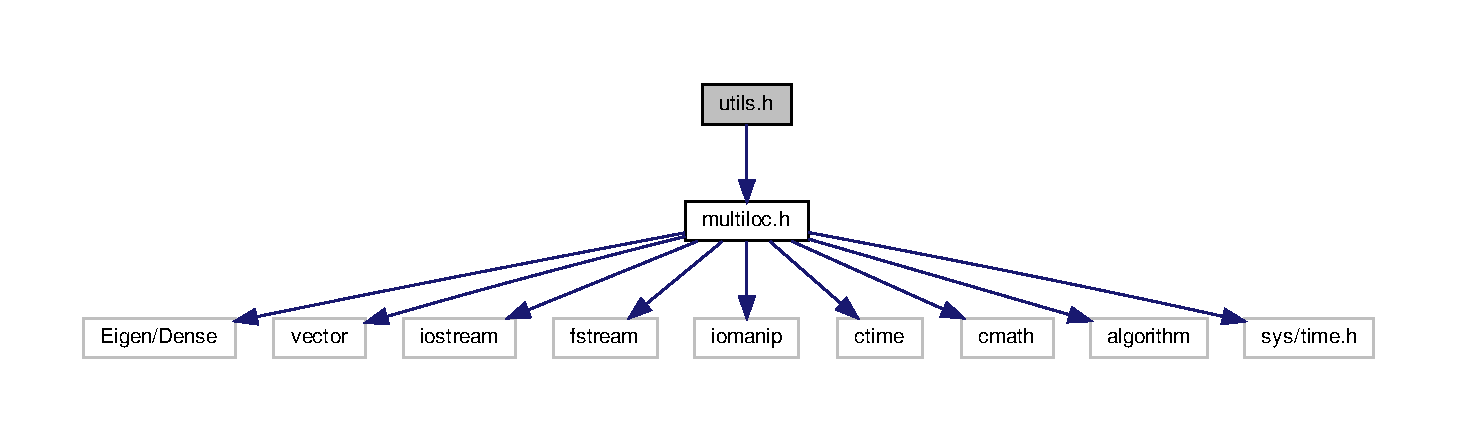
\includegraphics[width=350pt]{utils_8h__incl}
\end{center}
\end{figure}
\subsection*{Functions}
\begin{DoxyCompactItemize}
\item 
void \hyperlink{utils_8h_a30d9a377b4d890b95e9da3b0ad01b999}{print} (\hyperlink{multiloc_8h_a490e31016ad1c0d99b23e323d64e3aac}{one\+\_\+\+Tuple} \&list)
\begin{DoxyCompactList}\small\item\em 输出1维vector$<$double$>$的数据到命令行 \end{DoxyCompactList}\item 
void \hyperlink{utils_8h_af19e963b2af9ed4271dabf8ff5173a2a}{print} (\hyperlink{multiloc_8h_a2e41d128befae015727cbf20484696a9}{two\+\_\+\+Tuple} \&list)
\begin{DoxyCompactList}\small\item\em 输出2维vector$<$vector$<$double$>$$>$的数据到命令行 \end{DoxyCompactList}\item 
void \hyperlink{utils_8h_a6bf72582ec5cb8810d7f6a12f7e6a288}{print} (\hyperlink{multiloc_8h_aa614d5a3aa93583e717bf9a9c9b6627b}{three\+\_\+\+Tuple} \&list)
\begin{DoxyCompactList}\small\item\em 输出3维vector$<$vector$<$vector$<$double$>$$>$$>$的数据到命令行 \end{DoxyCompactList}\item 
void \hyperlink{utils_8h_ab41f9c53816779167ea445a169512601}{print} (Matrix\+Xd \&list, int \&total)
\begin{DoxyCompactList}\small\item\em 输出2维\+Matrix\+Xd前total个的数据到命令行 \end{DoxyCompactList}\item 
bool \hyperlink{utils_8h_a0f93995792a5f39c3ab0d5fe7513dc31}{read\+\_\+data} (const char $\ast$filename, \hyperlink{multiloc_8h_a490e31016ad1c0d99b23e323d64e3aac}{one\+\_\+\+Tuple} \&tuples)
\begin{DoxyCompactList}\small\item\em \+: 从文件中读取数据内容,将输出的结果保存在一维的vector$<$double$>$中. filename为需要读取数据的文件名路径,tuples保存读取的数据.读取数据成功,返回true.否则,返回false. \end{DoxyCompactList}\item 
bool \hyperlink{utils_8h_a8f7095b4f098b6f05662a5451211a653}{read\+\_\+file} (string \&Docement, \hyperlink{multiloc_8h_a490e31016ad1c0d99b23e323d64e3aac}{one\+\_\+\+Tuple} \&m\+\_\+data, \hyperlink{multiloc_8h_a2e41d128befae015727cbf20484696a9}{two\+\_\+\+Tuple} \&angle)
\begin{DoxyCompactList}\small\item\em 从文件中读取用于多目标定位的靶点和测向线信息,其中filename为需要读取数据的文件路径, 将读取的靶点坐标保存在m\+\_\+data中,将读取的测向线信息保存在angle中. \end{DoxyCompactList}\item 
bool \hyperlink{utils_8h_acbbdf84730da8712d34d2203a40e9d30}{read\+\_\+file} (string \&Docement, \hyperlink{multiloc_8h_a490e31016ad1c0d99b23e323d64e3aac}{one\+\_\+\+Tuple} \&m\+\_\+data, \hyperlink{multiloc_8h_a490e31016ad1c0d99b23e323d64e3aac}{one\+\_\+\+Tuple} \&angle)
\begin{DoxyCompactList}\small\item\em 从文件中读取用于单目标定位的靶点和测向线信息,其中filename为需要读取数据的文件路径, 将读取的靶点坐标保存在m\+\_\+data中,将读取的测向线信息保存在angle中. \end{DoxyCompactList}\end{DoxyCompactItemize}


\subsection{Function Documentation}
\index{utils.\+h@{utils.\+h}!print@{print}}
\index{print@{print}!utils.\+h@{utils.\+h}}
\subsubsection[{\texorpdfstring{print(one\+\_\+\+Tuple \&list)}{print(one_Tuple &list)}}]{\setlength{\rightskip}{0pt plus 5cm}void print (
\begin{DoxyParamCaption}
\item[{{\bf one\+\_\+\+Tuple} \&}]{list}
\end{DoxyParamCaption}
)}\hypertarget{utils_8h_a30d9a377b4d890b95e9da3b0ad01b999}{}\label{utils_8h_a30d9a377b4d890b95e9da3b0ad01b999}


输出1维vector$<$double$>$的数据到命令行 


\begin{DoxyParams}{Parameters}
{\em list为vector$<$double$>$类型} & \\
\hline
\end{DoxyParams}
\begin{DoxyReturn}{Returns}
无 
\end{DoxyReturn}
\index{utils.\+h@{utils.\+h}!print@{print}}
\index{print@{print}!utils.\+h@{utils.\+h}}
\subsubsection[{\texorpdfstring{print(two\+\_\+\+Tuple \&list)}{print(two_Tuple &list)}}]{\setlength{\rightskip}{0pt plus 5cm}void print (
\begin{DoxyParamCaption}
\item[{{\bf two\+\_\+\+Tuple} \&}]{list}
\end{DoxyParamCaption}
)}\hypertarget{utils_8h_af19e963b2af9ed4271dabf8ff5173a2a}{}\label{utils_8h_af19e963b2af9ed4271dabf8ff5173a2a}


输出2维vector$<$vector$<$double$>$$>$的数据到命令行 


\begin{DoxyParams}{Parameters}
{\em list为vector$<$vector$<$double$>$$>$类型} & \\
\hline
\end{DoxyParams}
\begin{DoxyReturn}{Returns}
无 
\end{DoxyReturn}
\index{utils.\+h@{utils.\+h}!print@{print}}
\index{print@{print}!utils.\+h@{utils.\+h}}
\subsubsection[{\texorpdfstring{print(three\+\_\+\+Tuple \&list)}{print(three_Tuple &list)}}]{\setlength{\rightskip}{0pt plus 5cm}void print (
\begin{DoxyParamCaption}
\item[{{\bf three\+\_\+\+Tuple} \&}]{list}
\end{DoxyParamCaption}
)}\hypertarget{utils_8h_a6bf72582ec5cb8810d7f6a12f7e6a288}{}\label{utils_8h_a6bf72582ec5cb8810d7f6a12f7e6a288}


输出3维vector$<$vector$<$vector$<$double$>$$>$$>$的数据到命令行 


\begin{DoxyParams}{Parameters}
{\em list为vector$<$vector$<$vector$<$double$>$$>$$>$类型} & \\
\hline
\end{DoxyParams}
\begin{DoxyReturn}{Returns}
无 
\end{DoxyReturn}
\index{utils.\+h@{utils.\+h}!print@{print}}
\index{print@{print}!utils.\+h@{utils.\+h}}
\subsubsection[{\texorpdfstring{print(\+Matrix\+Xd \&list, int \&total)}{print(MatrixXd &list, int &total)}}]{\setlength{\rightskip}{0pt plus 5cm}void print (
\begin{DoxyParamCaption}
\item[{Matrix\+Xd \&}]{list, }
\item[{int \&}]{total}
\end{DoxyParamCaption}
)}\hypertarget{utils_8h_ab41f9c53816779167ea445a169512601}{}\label{utils_8h_ab41f9c53816779167ea445a169512601}


输出2维\+Matrix\+Xd前total个的数据到命令行 


\begin{DoxyParams}{Parameters}
{\em list为\+Matrix\+Xd类型} & \\
\hline
{\em total为int类型} & \\
\hline
\end{DoxyParams}
\begin{DoxyReturn}{Returns}
无 
\end{DoxyReturn}
\index{utils.\+h@{utils.\+h}!read\+\_\+data@{read\+\_\+data}}
\index{read\+\_\+data@{read\+\_\+data}!utils.\+h@{utils.\+h}}
\subsubsection[{\texorpdfstring{read\+\_\+data(const char $\ast$filename, one\+\_\+\+Tuple \&tuples)}{read_data(const char *filename, one_Tuple &tuples)}}]{\setlength{\rightskip}{0pt plus 5cm}bool read\+\_\+data (
\begin{DoxyParamCaption}
\item[{const char $\ast$}]{filename, }
\item[{{\bf one\+\_\+\+Tuple} \&}]{tuples}
\end{DoxyParamCaption}
)}\hypertarget{utils_8h_a0f93995792a5f39c3ab0d5fe7513dc31}{}\label{utils_8h_a0f93995792a5f39c3ab0d5fe7513dc31}


\+: 从文件中读取数据内容,将输出的结果保存在一维的vector$<$double$>$中. filename为需要读取数据的文件名路径,tuples保存读取的数据.读取数据成功,返回true.否则,返回false. 


\begin{DoxyParams}{Parameters}
{\em } & \\
\hline
\end{DoxyParams}
\index{utils.\+h@{utils.\+h}!read\+\_\+file@{read\+\_\+file}}
\index{read\+\_\+file@{read\+\_\+file}!utils.\+h@{utils.\+h}}
\subsubsection[{\texorpdfstring{read\+\_\+file(string \&\+Docement, one\+\_\+\+Tuple \&m\+\_\+data, two\+\_\+\+Tuple \&angle)}{read_file(string &Docement, one_Tuple &m_data, two_Tuple &angle)}}]{\setlength{\rightskip}{0pt plus 5cm}bool read\+\_\+file (
\begin{DoxyParamCaption}
\item[{string \&}]{Docement, }
\item[{{\bf one\+\_\+\+Tuple} \&}]{m\+\_\+data, }
\item[{{\bf two\+\_\+\+Tuple} \&}]{angle}
\end{DoxyParamCaption}
)}\hypertarget{utils_8h_a8f7095b4f098b6f05662a5451211a653}{}\label{utils_8h_a8f7095b4f098b6f05662a5451211a653}


从文件中读取用于多目标定位的靶点和测向线信息,其中filename为需要读取数据的文件路径, 将读取的靶点坐标保存在m\+\_\+data中,将读取的测向线信息保存在angle中. 


\begin{DoxyParams}{Parameters}
{\em Docement为string类型} & \\
\hline
{\em m\+\_\+data为vector$<$double$>$类型} & \\
\hline
{\em angle为vector$<$vector$<$double$>$$>$类型} & \\
\hline
\end{DoxyParams}
\begin{DoxyReturn}{Returns}
bool类型,读取数据成功,返回true.否则,返回false. 
\end{DoxyReturn}
\index{utils.\+h@{utils.\+h}!read\+\_\+file@{read\+\_\+file}}
\index{read\+\_\+file@{read\+\_\+file}!utils.\+h@{utils.\+h}}
\subsubsection[{\texorpdfstring{read\+\_\+file(string \&\+Docement, one\+\_\+\+Tuple \&m\+\_\+data, one\+\_\+\+Tuple \&angle)}{read_file(string &Docement, one_Tuple &m_data, one_Tuple &angle)}}]{\setlength{\rightskip}{0pt plus 5cm}bool read\+\_\+file (
\begin{DoxyParamCaption}
\item[{string \&}]{Docement, }
\item[{{\bf one\+\_\+\+Tuple} \&}]{m\+\_\+data, }
\item[{{\bf one\+\_\+\+Tuple} \&}]{angle}
\end{DoxyParamCaption}
)}\hypertarget{utils_8h_acbbdf84730da8712d34d2203a40e9d30}{}\label{utils_8h_acbbdf84730da8712d34d2203a40e9d30}


从文件中读取用于单目标定位的靶点和测向线信息,其中filename为需要读取数据的文件路径, 将读取的靶点坐标保存在m\+\_\+data中,将读取的测向线信息保存在angle中. 


\begin{DoxyParams}{Parameters}
{\em Docement为string类型} & \\
\hline
{\em m\+\_\+data} & 为vector$<$double$>$类型 \\
\hline
{\em angle} & 为vector$<$double$>$类型\\
\hline
\end{DoxyParams}
\begin{DoxyReturn}{Returns}
bool类型,读取数据成功,返回true;否则,返回 false。 
\end{DoxyReturn}

%--- End generated contents ---

% Index
\backmatter
\newpage
\phantomsection
\clearemptydoublepage
\addcontentsline{toc}{chapter}{Index}
\printindex

\end{document}
